In this section we review the related work with respect to relevant frameworks and concepts used in this paper.

\subsection{Spark}
Apache Spark is an efficient and general-purpose cluster computing system. It provides APIs for Java, Scala, Python and R. Spark runs an optimized engine that supports general execution graphs. Besides the core Spark, there are further high-level tools to support mining of large data sets as illustrated on Figure~\ref{fig:spark}. Spark SQL is built for SQL and structured data processing, MLlib for machine learning, GraphX for graph processing, and Spark Streaming for processing data that is continuously generated by different sources.
\begin{figure}[h]
    \centering
    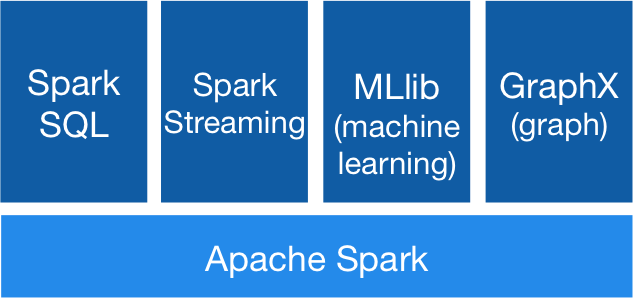
\includegraphics[width=0.45\textwidth]{images/spark-stack}
    \caption{Spark stack (Source: \cite{spark})}
    \label{fig:spark}
\end{figure}

Another great advantage of Spark is that it runs with Hadoop, Mesos, standalone, or in the cloud. It can access wide rage of external data sources including Hadoop file system (HDFS), Cassandra, HBase, and S3. 

It also has up to 100 times shorter run-time than Hadoop MapReduce in memory, or 10 times shorter on disk. The reason for this is that Apache Spark has an advanced Directed Acyclic Graph(DAG) execution engine that supports acyclic data flow and in-memory computing.\cite{spark}

To be more efficient, Spark also offers an abstraction called resilient distributed data set (RDD). RDDs can be stored in memory between queries without the need for replication. Instead, the lost data is only rebuilt on failure using lineage graph, meaning that each RDD remembers how it was built and is able to rebuild itself resulting in a more fault-tolerant application. RDDs are one of the main reasons that make it possible for Spark to outperform existing big data processing frameworks. \cite{spark}

Based on \cite{spark:rdds}, RDDs can be created from parallelized collections or from external data sources like Hadoop File System (HDFS), PostgreSQL or S3. They support two types of operations; transformation and actions.

Transformations create new RDDs from existing ones and they are executed only on demand, i.e. they are executed lazily. However, lazy evaluation has its drawbacks, namely that many partitions\footnote{By default RDDs are partitioned automatically  through different nodes with preset number of partitions. Usually 2-4 partitions per computational unit.} are computed multiple times resulting in longer execution time. A solution to these is RDD persistence with different levels (main memory, local disk or mixed), which means caching RDDs in memory across different operations. 
 
In contrast with transformations, actions launch a computation to return a final value to the program or write data to external storage. Actions triggers execution using lineage graph to load the data into original RDD, carry out all transformations and return  results to the driver program or write it out to file system as shown on Figure \ref{fig:spark-ops}.

\begin{figure}[h]
    \centering
    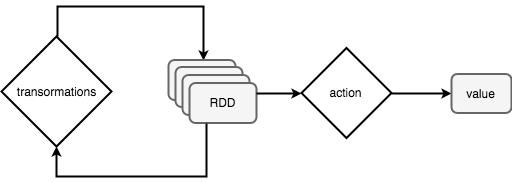
\includegraphics[width=0.5\textwidth]{images/operations_spark.png}
    \caption{Operations on RDDs in Spark}
    \label{fig:spark-ops}
\end{figure}

As illustrated on Figure~\ref{fig:spark-cluster} Spark applications run as independent sets of processes on a cluster, navigated by the SparkContext object in the main program, which is called the driver program. The cluster managers allocate resources across applications. There are three types of cluster managers that the SparkContext can connect to:
\begin{enumerate}
\item Apache Mesos, a general cluster manager, 
\item Spark's own built-in cluster manager and
\item YARN, which is the resource manager in Hadoop.
\end{enumerate}
After the connection is established, Spark acquires executors on nodes of the cluster. The executors are processes that run computations and store data for the application. SparkContext sends the application code and tasks to the executors to run.
\cite{spark-cluster}

\begin{figure}[h]
    \centering
    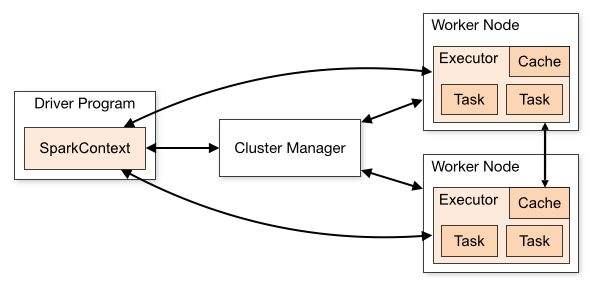
\includegraphics[width=0.5\textwidth, height=5cm]{images/cluster-overview}
    \caption{Running Spark on a cluster (Source: \cite{spark-cluster})}
    \label{fig:spark-cluster}
\end{figure}

\subsection{PySpark}
To enable data scientists to leverage the value of big data, Spark added a Python API (also known as PySpark) with support for built-in Spark functions and an interface for native Python code called user-defined functions (UDFs), which transform values from a single row within a table to produce a single corresponding output value per row.

PySpark is built on top of Spark's Java API. Data is processed in Python and cached or shuffled in the Java Virtual Machine (JVM). As seen in Figure \ref{fig:pyspark}, in the Python driver program, the SparkContext uses Py4J\footnote{Py4J enables Python programs running in a Python interpreter to dynamically access Java objects in a Java Virtual Machine. For more details see \url{https://www.py4j.org/}} to launch a JVM and create a JavaSparkContext. Py4J is only used on the driver for local communication between the Python and Java SparkContext objects; large data transfers are performed through a different mechanism.
\begin{figure}[h]
    \centering
    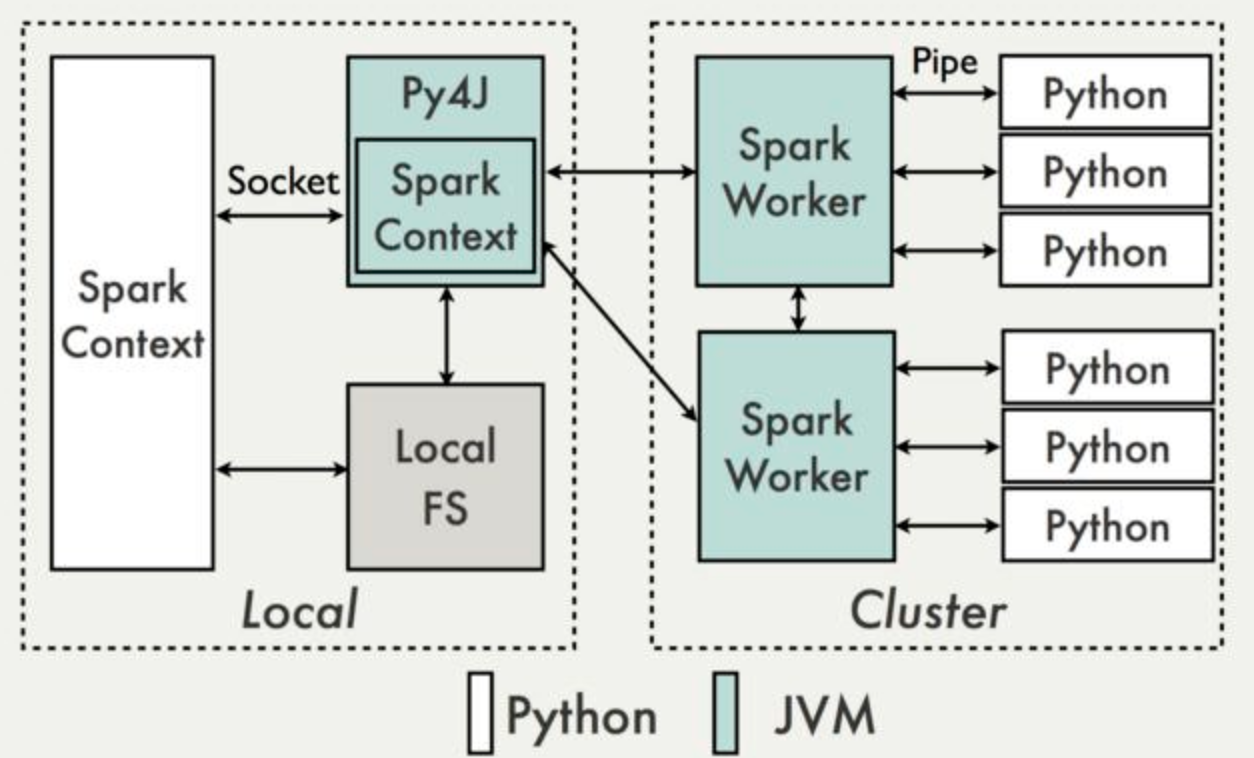
\includegraphics[width=0.45\textwidth]{images/pyspark.png}
    \caption{PySpark internal structure}
    \label{fig:pyspark}
\end{figure}

There are two main limitations of UDFs in PySpark: the scalar computational model and inefficient data movement between Java and Python resulting in serialization overhead. What is more, UDFs are practically black-boxes for the Spark execution engine so there is no additional optimization. 

To avoid the poor performance UDFs, one can use the available operations on Spark DataFrames, which are more efficient as the Python calls are translated into SQL query plans in the JVM. 

In Spark 2.3.0 Pandas UDFs have been introduced. Pandas UDFs are executed by Spark using Arrow\footnote{Apache Arrow is a cross-language development platform for in-memory data. For more details refer to \url{https://arrow.apache.org/}} to transfer data and then Pandas to process the transferred data. Currently, there are two types of Pandas UDFs: Scalar and Grouped Map. Scalars are used for vectorizing scalar operations and thus eliminating the need to iterate over all rows as with standard UDFs. Grouped map Pandas UDFs implement the "split-apply-combine" pattern and can be used for for group level operations.\cite{spark-sql}

\subsection{Parquet}
Apache Parquet is a columnar storage format. It is available in the Hadoop ecosystem with every data processing framework, data model or programming language. It is built to support highly efficient compression and encoding schemes. It has been demonstrated that the performance is heavily dependant on applying the right compression and encoding scheme to the data. Compression schemes can be specified on a per-column level in Parquet and allows adding more encoding schemes as they are invented and implemented.
\cite{parquet}

Parquet is slow to write, but it is very fast to read as it is optimized for the \textit{write once read many} paradigm. If you only access a subset of the total columns then Parquet can be even more efficient than some other record oriented storage formats, such as .csv where the whole file needs to be read first. 

Parquet supports partitioning, which is a technique for physically dividing the data during loading, based on values from one or more columns, to speed up queries regarding those columns. This comes very handy in a distributed file system, such as HDFS.

Parquet storage format works very smoothly with Spark SQL - saving both time and space - as compression minimizes size of files by 75\% on average, columnar format allows reading only selective records, and reduced size of input data directly impacts the Spark DAG scheduler's decision on execution graphs. \cite{ibm_parquet}

\subsection{Containerization}
Using Linux containers to deploy applications is called containerization. In the recent years it has become increasingly popular thanks to Docker, which is a platform to develop, deploy, and run applications with containers. It is developed to build, secure and manage different applications from development to production both on premises and in the cloud. Developing with Docker containers is flexible, scalable, portable and lightweight.

A container is launched by running an image, which is an executable package that has everything that is required to run the application. The code, a runtime, libraries, environment variables, and configuration files. The container can be referred to as a runtime instance of the respective image. A container runs on Linux and shares the kernel of the host machine with other containers. It runs a discrete process, taking no more memory than any other executable, making it lightweight compared to a virtual machine.\cite{docker}